\section{Ball Swinging in a Horizontal Circle}

\begin{overview}

	\textbf{Overview:} Remember the Mass Swinging in a Horizontal Circle in Activity \ref{MassCircle}? We already started analyzing the forces acting on the ball in that activity. Now that we have another model in our tool bag, we return to this scenario to continue our analysis of the forces on the ball.
	
\end{overview}

\noindent\textbf{Phenomenon:} Ball on a string, swinging in a horizontal circle at constant speed. The experiment shows that as the ball moves faster, $\theta$ becomes larger, and the tension in the string increases.

%\begin{wrapfigure}[6]{r}{6cm}
%        \centering
%        \vspace{-\baselineskip}
\begin{center}
			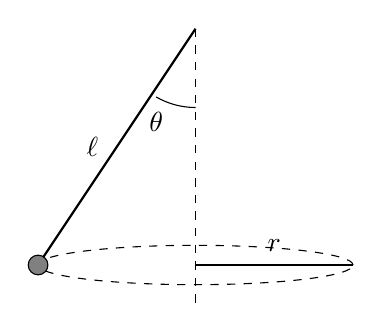
\begin{tikzpicture}{r}{1}
				% Reference Measurements
				\draw[dashed] (2,3.5) -- (2,0);
				\draw[dashed] (2,0.5) ellipse (2cm and 0.25cm);
				\draw[thin] (2,0.5) -- (4,0.5) node[midway,above=1.5pt] {$r$};
				\draw[thin] (2,2.5) arc (270:240:1) node[below=2pt] {$\theta$};
				
				% Ball & String
				\draw[thick] (2,3.5) -- (0,0.5) node[midway,left=3pt] {$\ell$};
				\draw[fill=gray] (0,0.5) circle (0.125cm);
			\end{tikzpicture}
\end{center}
%	  \end{wrapfigure}


\subsection*{What model/approach would you use?}

Suppose you are interested in how the tension in the string depends on the angle $\theta$ that the string makes with the vertical direction. Which approach do you think would help you make progress with this question: energy conservation, momentum %or angular momentum
conservation, or Newton's 2nd law?\\

\noindent Discuss in your group what information you specifically need, and which models/approaches can give you that information. Start by thinking about the specific motion and what is required to produce this motion. (Note that rotational velocity -- how fast the ball swings around the circle -- is assumed constant. What does this imply?)

\subsection*{Use the model}

Carry out the analysis using whichever approach/model you have decided on.
\begin{enumerate}
	\item Put a properly labeled \forcediag{} for the ball on the board.
	\label{act8.3.1-2a}
	
	\item Use the \forcediag{} to develop \textbf{two} mathematical relationships (one for the vertical direction and one for the horizontal direction). You will need to figure out (or remember) the direction of the acceleration of an object traveling in a circle at constant speed. The magnitude of this acceleration is $a_\text{centripetal} = \frac{v_\text{tangential}{}^2}{r}$.\\(Notice $v_\text{tangential}$ refers to the \emph{tangential} speed of the ball).
	
	\item Does the force of the string on the ball equal the force of the Earth on the ball? If not, what does?
	
\WCD
\vspace{2pt}

	\item Illustrate using vectors what happens to the tension in the string ($\vec{F}_\text{string on ball}$) when the tangential speed of the ball increases. Think about how the two relationships in \eqref{act8.3.1-2a} can both be satisfied.
	
	\item Develop a short explanation of why the angle of the string (from the vertical direction) changes when the tangential velocity is increased significantly. Check this out with the real ball and string.
\end{enumerate}

\WCD
